\documentclass[11pt,a4paper]{article}
\usepackage[margin=2.4cm]{geometry}
\usepackage{amsmath,amssymb,graphicx,booktabs,microtype}
\usepackage[colorlinks=true,linkcolor=blue!60!black,citecolor=blue!60!black,urlcolor=blue!60!black]{hyperref}
\usepackage{xcolor}
\newcommand{\todo}[1]{{\color{red}[#1]}}
\providecommand{\AuthorName}{Joseph Foe}
\providecommand{\AuthorEmail}{foe.joseph@gmail.com}
\newcommand{\Hess}{\mathrm{Hess}\,}
\newcommand{\esc}{{\rm esc}}
\newcommand{\YM}{{\rm YM}}

\title{The Lee--Wick ghost of Yang--Mills mechanics is malicious at every energy:\\
a parameter-free $E^{9/4}$ instability law and an area-filling escape landscape}

\author{\AuthorName\\ \small \texttt{\AuthorEmail}}
\date{\today}

\begin{document}
\maketitle

\begin{abstract}
Quadratic gravity is renormalisable but propagates a massive spin-2 ghost, and every proposed
quantum cure (fakeons, Lee--Wick prescriptions, Merlin modes) inherits a prior classical question:
does the interacting Ostrogradsky ghost run away? We study the closest tractable analogue in which
the interactions are fixed by gauge symmetry rather than chosen: SU(2) Lee--Wick Yang--Mills theory
on a spatial three-torus, restricted to its spatially homogeneous (zero-momentum), colour-diagonal
sector, an exact twelve-dimensional Hamiltonian system consisting of chaotic Yang--Mills mechanics coupled to a wrong-sign oscillator.
The ghost-free manifold is invariant, and its transverse Lyapunov exponent $\lambda_\perp(E)$ is
positive at every energy tested, down to $E=0.008$ in units $g=M=1$, with no threshold and no
exponential suppression. At low energy the growth is parametric resonance driven by the
transverse oscillations of the chaotic flow inside the Yang--Mills channels, and we derive the
resulting law: the uniform microcanonical measure on the two transverse channel actions, together
with adiabatic in-channel motion, gives a $u^{-6}$ spectral tail (measured exponent $-6.0$) and
hence $\lambda\propto E^{9/4}$, with the prefactor fixed by the classical density of states,
$\lambda_{\rm diag}=(32\pi^3/105\sqrt2)\,E^{9/4}/Z=0.0120\,E^{9/4}$ with $Z=557.1$. The
single-mode rate measured directly at $E=0.008$, $0.015$, $0.02$ and $0.03$ is
$(0.0120\pm0.0003)\,E^{2.24\pm0.03}$, i.e.\ the prediction is reproduced at each energy to
within $3\%$ with no adjustable parameter, and to within $10\%$ up to $E=0.1$; the physical three-component ghost lies a factor
$1.7$--$2.3$ above it over the same range, converging towards it from above as the mode-mixing
contribution fades. Nonlinearly the ghost escapes to a
finite-time singularity through a self-accelerating tachyonic loop, and the escape-time landscape
over initial conditions is fractal with uncertainty exponent $\alpha\simeq0.05$, i.e.\ boundary
dimension $\simeq1.95$, on every section examined and down to $10^{-14}$ of the section width:
the ghost-free manifold is a repeller with no open basin. We discuss what this implies for the
classical limit of the fakeon prescription and for the epoch in which such a ghost could have
mattered cosmologically.
\end{abstract}

\section{Introduction}

Perturbative quantum gravity built on the Einstein--Hilbert action is not renormalisable; adding
the curvature-squared invariants with dimensionless coefficients makes it so \cite{Stelle77}, at
the price of a massive spin-2 field with a wrong-sign kinetic term. Quantised as an ordinary
particle this ghost forces a choice between negative norms and an unstable vacuum, and a number of
programs attempt to keep Stelle's renormalisability without the pathology: Anselmi's fakeons
\cite{Anselmi17,Anselmi18}, in which the ghost is quantised with an averaged $\pm i\epsilon$
prescription and never appears in asymptotic states; Lee--Wick-type prescriptions
\cite{LeeWick,GOW08}; the Merlin modes of Donoghue and Menezes \cite{DonoghueMenezes}; agravity
\cite{SalvioStrumia}. All of these are statements about the quantum theory. They inherit a
classical question: any non-degenerate higher-derivative Lagrangian has an Ostrogradsky
Hamiltonian unbounded below, and the naive expectation is that interactions let energy flow
without limit between the ghost and the normal sector. Recent work has shown that this expectation
is not a theorem: interacting ghost systems can be globally stable or ``benign''
\cite{DMV22,DamourSmilga,Smilga}, but essentially all such examples use scalar toy models whose
interactions were chosen to be stable, and several are integrable or close to it.

Here we study the classical question in a system where the interactions are dictated by a gauge
symmetry and the normal sector is chaotic. Lee--Wick Yang--Mills theory,
\begin{equation}
\mathcal L=-\tfrac14F^a_{\mu\nu}F^{a\mu\nu}+\frac1{2M^2}(D^\mu F_{\mu\nu})^a(D_\rho F^{\rho\nu})^a,
\label{eq:LWYM}
\end{equation}
is the gauge-theory counterpart of the Weyl-squared term (the same operator appears in the
Lee--Wick Standard Model \cite{GOW08}); it propagates a massive spin-1 ghost of mass $M$ alongside
the massless gluon. We place the theory on a spatial three-torus $T^3$ of side $L$, so that
spatially homogeneous fields are the zero-momentum sector of a finite-volume system, the setting
of L\"uscher's small-volume analysis \cite{Luscher83}, rather than an idealisation in infinite
space. Restricted to that sector in the colour-diagonal ansatz the theory
reduces to an exact twelve-dimensional Hamiltonian system \cite{note:derive}: Yang--Mills
mechanics \cite{MatinyanSavvidy,Savvidy}, which is chaotic on almost all of phase space at every
energy (the regular islands \cite{DahlqvistRussberg} have small measure, and by the scaling
symmetry the same fraction at every $E$), coupled to a three-component ghost. Because the sector is exact, instability here is an existence proof of
instability of the full classical theory on the torus (the converse would not have held).

Our results are as follows. (i) The ghost-free manifold is invariant and its transverse
Lyapunov exponent is positive at every energy tested, down to $E=0.008$ in the natural units,
following a power law close to $E^{9/4}$ at low energy
(Sec.~\ref{sec:lambda}). (ii) The exponent $9/4$ and the prefactor of the single-mode
(``diagonal'') rate are derived from the channel statistics of Yang--Mills mechanics and the
classical density of states, with no free parameter, and the derived law
$0.0120\,E^{9/4}$ is reproduced by direct measurement to within $3\%$ at four energies
(Sec.~\ref{sec:derivation}). In particular the absence of exponential suppression follows from the
microcanonical measure on small transverse actions being a power law. (iii) Nonlinearly the ghost
escapes to a finite-time singularity through an identified mechanism, and the escape-time
landscape over initial conditions is fractal with boundary dimension $\simeq1.95$ on every
section examined (Sec.~\ref{sec:nonlinear}). (iv) On periodic orbits the ghost is Floquet-stable
in most of the energy range, including energies at which its mass matrix is transiently negative
(Sec.~\ref{sec:floquet}); these are the only exact invariant sets on which a ghost can sit, and
they are unstable within the base flow. Sec.~\ref{sec:discussion} discusses the implications for
the fakeon classical limit and the cosmological scaling of the instability rate.

\section{The model}
\label{sec:model}

On $T^3$ with periodic boundary conditions, with $A^a_i=\delta^a_i q_i(t)$ in temporal gauge and
$A_0=0$, the Gauss-law constraint and the six off-diagonal colour equations vanish identically on
the ansatz, symmetric criticality holds, and the action is $L^3\!\int dt\,L_{\rm red}$ with
\cite{note:derive}
\begin{equation}
L_{\rm red}=\tfrac12|\dot q|^2-V(q)-\frac1{2M^2}\,\big|\ddot q+\nabla V(q)\big|^2,\qquad
V(q)=\tfrac{g^2}2\,(x^2y^2+y^2z^2+z^2x^2).
\label{eq:Lred}
\end{equation}
The volume factor $L^3$ multiplies the whole action and drops out of the equations of motion; the
energies quoted below are energy densities, the total energy on the torus being $L^3E$. The ghost
amplitude is literally the violation of the ordinary Yang--Mills equation of motion.
The rescaling $t\to t/M$, $q\to(M/g)q$ gives $L=(M^4/g^2)\tilde L$ with $g=M=1$; henceforth time
is in units of $1/M$, fields in units of $M/g$, and energy in units of $M^4/g^2$. With the
auxiliary field $w=\ddot q+\nabla V$ the dynamics is generated by the separable Hamiltonian
\begin{equation}
H=\tfrac12|P|^2-\tfrac12|W|^2+V(q)+w\cdot\nabla V(q)-\tfrac12|w|^2,\qquad q=p-w,
\label{eq:H}
\end{equation}
with $\dot p=P$, $\dot w=-W$, $\dot P=-\partial_pU$, $\dot W=-\partial_wU$. The state is
$(p,w,P,W)$, four 3-vectors. Two structural facts make the problem sharp:
\begin{itemize}
\item $w=W=0$ is an invariant submanifold on which the dynamics is exactly Yang--Mills mechanics,
$\ddot p=-\nabla V(p)$, whose maximal Lyapunov exponent scales exactly as
$\lambda_\YM\simeq0.38\,E^{1/4}$ by the absence of an intrinsic scale.
\item Linearised about it, the normal sector decouples and the ghost obeys
\begin{equation}
\ddot w=-\big(1+\Hess V(p(t))\big)\,w ,
\label{eq:hill}
\end{equation}
a Hill-type equation with chaotic rather than periodic coefficients: a product of random
matrices in the Furstenberg sense. Its largest Lyapunov exponent $\lambda_\perp(E)$ is the
transverse Lyapunov exponent of the ghost-free manifold in the sense of the theory of riddled
basins and blowout bifurcations \cite{OttSommerer,ABS96}.
\end{itemize}
The eigenvalues of $\Hess V$ satisfy $\lambda_{\min}\ge-\sqrt{2V}$ with equality on the ridges
$x=\pm y$, $z=0$ (and permutations), so the ghost mass matrix $1+\Hess V$ can become non-positive
only for $E\ge\tfrac12$ (a trajectory at rest on a ridge with $V=E$). Inside a channel
($|x|\gg|y|,|z|$) the negative eigenvalue is $\approx-3y^2$ and shrinks with depth; the
tachyonic configurations lie near turning points on the ridges between channels, not deep inside
them. Below $E=\tfrac12$ the instability, if any, must be parametric.

\section{Numerical methods}
\label{sec:methods}

All integrations use a fourth-order Yoshida symplectic scheme \cite{Yoshida} for the separable
Hamiltonian (\ref{eq:H}) or its linearisation. Yang--Mills trajectories with small transverse
action travel far along the channels, where the transverse frequency is $\sim|x|$; a fixed-step
scheme becomes unstable at $|x|\,dt\gtrsim1.57$, and channel depths are heavy-tailed (at $E=1$
the maximum of $|p|$ over $400$ time units has median $10$, 99th percentile $80$, and exceedance
$\propto D^{-2}$), so every trajectory is sub-stepped individually whenever
$\max_i|p_i|\,dt>0.25$. Relative energy errors stay at $\sim10^{-3}$ over $T=7\times10^4$.

$\lambda_\perp$ is estimated from the slope of the accumulated log-growth of the renormalised
ghost vector $(w,\dot w)$ over the trailing half of the run, with an adaptive stopping rule on
the ensemble standard error, the block-to-block drift and an $a+b/T$ trend extrapolation; the
difference between the final estimate and the extrapolation ($\le2.5\%$ for $E\ge0.015$,
$\le10\%$ at $E=0.008$) is quoted as the systematic uncertainty, the statistical standard error
being much smaller. For the physical ghost the norm of the full six-component vector is
renormalised, which is the standard estimator of the largest exponent of the coupled system. For
the ``diagonal'' ghost of Sec.~\ref{sec:lambda}, in which the three components are independent
scalar oscillators, each component is renormalised separately and the three log-growths are
averaged: the exponent of the single-mode mechanism is the mean of three realisations of the same
scalar process, not their maximum.\footnote{Renormalising the norm of the three-vector instead
returns, at finite $T$, the largest of three finite-time exponents. At these run lengths the
finite-time exponent distribution is wide (standard deviation $2$--$5$ times the mean,
$30$--$40\%$ of individual trajectories with negative finite-time slope at $E\le0.03$), and the
maximum of three overestimates the mean by a factor $1.5$--$1.7$ over $E=0.008$--$0.03$,
decreasing to $1.1$ at $E=1$ as the finite-time distribution narrows. An earlier version of this work used that estimator and reported a corresponding
$30$--$50\%$ excess over Eq.~(\ref{eq:final}).} Ensembles of
$10^3$ (CPU) to $2\times10^5$ (GPU) trajectories were used; the GPU code integrates each
trajectory inside a single kernel. Initial data are random phase points rescaled to the energy
shell by the scaling symmetry, with a burn-in of $200$ Yang--Mills times ($200\,E^{-1/4}$;
doubling or quartering it does not change the converged exponents). The instability is an
ensemble-mean statement: at $E=0.008$ the finite-time slopes of individual trajectories over
$T\sim10^5$ have a standard deviation several times the mean, and roughly $40\%$ of them are
negative, as expected for a wide finite-time Lyapunov distribution with a positive mean. Two
implementations (numpy on CPU, CuPy on GPU) were used for the production runs. In addition, the
channel statistics of Sec.~\ref{sec:derivation}, the Hessian spectrum, the transverse exponents
for $E\ge0.215$, the Floquet tongues of Sec.~\ref{sec:floquet}, the escape statistics of
Sec.~\ref{sec:nonlinear} and the full-system Lyapunov exponent were reproduced with a third,
separately written integrator; where a number below comes from that re-run it is said so.

The nonlinear escape-time landscape (Sec.~\ref{sec:nonlinear}) uses the same integrator on the
full system with escape declared at $\max|{\rm component}|>10^4$, about one time unit before the
singularity; only the ordering of escape times between nearby initial conditions matters, so the
same $dt$ and threshold are used throughout. Growth laws of individual escaping trajectories were
confirmed with an adaptive DOP853 integration at tolerance $10^{-11}$. The code (numpy, C/OpenMP and CUDA
implementations, the symbolic reduction, the analysis scripts and the data behind every figure and
table) is at \url{https://github.com/foejoseph-lab/hdym}.

\section{The transverse Lyapunov exponent}
\label{sec:lambda}

\begin{figure}
\centering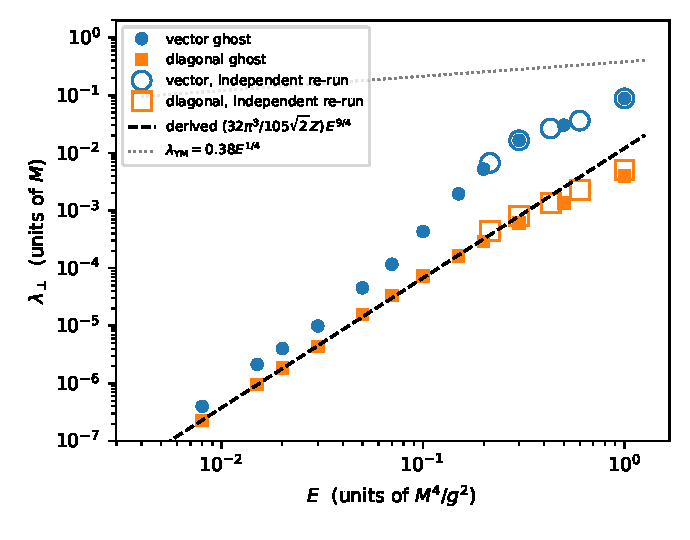
\includegraphics[width=.6\textwidth]{fig_lambda.pdf}
\caption{Transverse Lyapunov exponent of the ghost-free manifold. Circles: physical
three-component ghost; squares: ``diagonal'' ghost in which the off-diagonal entries of
$\Hess V$ are dropped (three independent scalar oscillators, per-component estimator of
Sec.~\ref{sec:methods}). Dashed: the parameter-free prediction of Sec.~\ref{sec:derivation} for
the diagonal ghost, $(32\pi^3/105\sqrt2)\,E^{9/4}/Z=0.0120\,E^{9/4}$ with $Z=557.1$; nothing is
fitted. Dotted: the Yang--Mills Lyapunov exponent for comparison. Filled symbols: GPU production
runs ($N=2\times10^5$ at $E\le0.03$, $10^5$ above). Open symbols: the independent re-run of
Sec.~\ref{sec:methods} at $E=1$, $0.6$, $0.43$, $0.3$ and $0.215$ ($512$ trajectories each);
its diagonal-ghost points use the three-vector norm estimator and lie above the per-component
values by the $1.1$--$1.3$ expected at these energies (footnote in Sec.~\ref{sec:methods}).}
\label{fig:lambda}
\end{figure}

Figure~\ref{fig:lambda} shows $\lambda_\perp(E)$. It is positive at every energy from $E=1$ down
to $E=0.008$. Table~\ref{tab:low} lists the four lowest energies, at which both the physical
ghost and the diagonal ghost were measured with $N=2\times10^5$ trajectories and run lengths
$T=1.2$--$1.8\times10^5$ (the same Yang--Mills ensembles for both). At $E=0.015$ the physical
value $2.13\times10^{-6}$ agrees with three earlier independent runs ($2.08$--$2.35\times10^{-6}$;
CPU $N=1024$, $T=5.4\times10^4$; GPU short and long). Positivity at the lowest energies does not
rest on the transient part of the estimate: runs at $T=2.6\times10^4$ and $5.4\times10^4$ agree
within $10\%$, whereas a bounded ghost would give a ratio of $0.48$, and the per-trajectory
log-growth is linear in $T$ over the whole trailing half of every run.

\begin{table}
\centering
\caption{Transverse Lyapunov exponents at the four lowest energies ($N=2\times10^5$). The
diagonal-ghost column is the single-mode rate (per-component estimator); the last column is its
ratio to the parameter-free prediction (\ref{eq:final}), $0.0120\,E^{9/4}$. Uncertainties are
the gap between the final estimate and the $a+b/T$ extrapolation; statistical standard errors
are $0.2$--$3\%$.}
\label{tab:low}
\begin{tabular}{ccccc}
\toprule
$E$ & $\lambda_\perp$ (vector) & $\lambda_{\rm diag}$ & vector/diag & $\lambda_{\rm diag}/0.0120E^{9/4}$\\
\midrule
$0.03$  & $9.92\times10^{-6}$ & $4.36\times10^{-6}$ & $2.27$ & $0.971$\\
$0.02$  & $4.02\times10^{-6}$ & $1.84\times10^{-6}$ & $2.18$ & $1.021$\\
$0.015$ & $2.13\times10^{-6}$ & $9.47\times10^{-7}$ & $2.25$ & $1.002$\\
$0.008$ & $4.00\times10^{-7}\,(\pm4\%)$ & $2.29\times10^{-7}\,(\pm10\%)$ & $1.75$ & $0.995$\\
\bottomrule
\end{tabular}
\end{table}

Over $0.008\le E\le0.03$ the diagonal ghost follows
\begin{equation}
\lambda_{\rm diag}=(0.0114\pm0.0010)\,E^{2.24\pm0.03},
\qquad\text{equivalently}\qquad
\lambda_{\rm diag}=(0.0120\pm0.0003)\,E^{9/4}
\label{eq:fit}
\end{equation}
with the exponent fixed at $9/4$; the local slopes between successive points being $2.26$, $2.32$ and $2.13$. The physical ghost
lies a factor $2.2$--$2.3$ above it at $E=0.015$--$0.03$ and $1.75$ at $E=0.008$, with a local
slope of $2.66$ between the two lowest points; the excess $\lambda_\perp-\lambda_{\rm diag}$
falls faster than $E^{9/4}$, so the asymptotic law for the physical ghost is the diagonal one.
There is no threshold. Over the factor-of-four range of Table~\ref{tab:low} an exponential law
$\exp(-cE^{-1/4})$ with $c\simeq3.5$ has a comparable local slope, so the fit alone does not
exclude exponential suppression; that exclusion comes from the spectral analysis of
Sec.~\ref{sec:derivation}, and the parameter-free agreement of the diagonal rate with
(\ref{eq:final}) at four energies is the quantitative form of it.

Two further features of the curve are diagnostic. First, $\lambda_\perp(E)$ is not a single power
law: it steepens between $E\simeq0.1$ and $0.25$, flattens between $0.3$ and $0.6$, and steepens
again above $0.6$ (in the re-run the local logarithmic slope is $2.7$ between $0.215$ and $0.3$,
$1.3$ and $0.9$ between $0.3$ and $0.6$, and $1.7$ between $0.6$ and $1$). Second, the ratio
between the physical vector ghost and the diagonal ghost (off-diagonal Hessian entries dropped)
is $22$ at $E=1$, $27$ at $0.3$, $18$ at $0.2$, $12$ at $0.15$, $5.9$ at $0.1$, $2.9$ at $0.05$,
$2.2$--$2.3$ at $0.015$--$0.03$ and $1.75$ at $0.008$ (re-run, norm estimator for the diagonal
ghost: $15$--$21$ over $E=0.215$--$1$).
The reading is that
above $E\sim0.1$ the growth is dominated by mixing of the three degenerate ghost modes by the
off-diagonal entries in the interior of the potential, while the low-energy power law is
single-mode parametric driving by the diagonal entries; the steepening between $0.1$ and $0.25$
is the mixing contribution switching off. The re-steepening above $0.6$ coincides with the exact
tachyonic threshold $E=\tfrac12$: the fraction of time with a non-positive ghost mass matrix
vanishes identically below $E=\tfrac12$ (measured zero at $E=0.43$), is $0.13\%$ at $E=0.6$, and
rises to $3\%$ at $E=1$.

\section{Derivation of the $E^{9/4}$ law}
\label{sec:derivation}

\subsection{Spectral formula and the $u^{-6}$ tail}

Because Yang--Mills mechanics is scale-free, the Hessian along a trajectory at energy $E$ is
$\Hess V(t;E)=E^{1/2}h(E^{1/4}t)$ with $h$ computed once at $E=1$. Equation (\ref{eq:hill}) is
then a unit-frequency oscillator driven parametrically by a stationary process of strength
$E^{1/2}$ and correlation time $E^{-1/4}$. For weak driving, the Lyapunov exponent of a randomly
modulated oscillator $\ddot w+(1+\xi(t))w=0$ is \cite{APW86,Jarzynski93}
$\lambda=\tfrac18S_\xi(2)$, with $S_\xi(\omega)=\int\langle\xi(\tau)\xi(0)\rangle e^{i\omega\tau}
d\tau$ the two-sided spectrum. Hence
\begin{equation}
\lambda_\perp(E)\simeq\tfrac18\,E^{3/4}\,\hat s\!\big(2E^{-1/4}\big),
\label{eq:spectral}
\end{equation}
where $\hat s(u)$ is the spectrum of the relevant Hessian entry at $E=1$. This is the classical
statement that a fast oscillator coupled to a slow chaotic system responds to the chaotic
spectrum at its own (doubled) frequency \cite{Ott79,Jarzynski93}; the ghost is that result with
the sign of the response reversed. It is also the Thouless/Born formula for the inverse
localisation length of a one-dimensional Anderson problem in the time domain, with $\lambda_\perp$
the inverse localisation length and the Hessian the (correlated) disorder.

The measured spectrum of the diagonal entries at $E=1$ has a power-law tail. A first estimate
(512 trajectories, no ghost) gave $\hat s\propto u^{-5.6\ {\rm to}\ -6.2}$ over $u=6$--$30$ with
a local exponential rate that keeps falling ($1.5\to0.23$); a high-statistics multitaper
estimate (DPSS, $NW=16$, $K=8$; $2048$ trajectories, $T=2\times10^4$, $98\,304$ segments of
$409.6$ time units) of the mean diagonal entry gives local slopes $-6.14$, $-6.05$, $-6.00$,
$-5.98$, $-5.89$ over $u=5$--$8$, $8$--$12$, $12$--$20$, $20$--$30$, $30$--$45$, and
\begin{equation}
u^6\,\hat s(u)=A=21.6\pm0.3\qquad(u=8\text{--}45),
\label{eq:A}
\end{equation}
constant to $\pm1\%$; beyond $u\simeq45$ the ensemble runs out of sufficiently deep visits. It
is not an exponential. Splitting the segments by their deepest excursion confirms the kinematic
origin of the tail: segments whose maximum $|p|$ is below the median ($10.0$) reproduce the total
spectrum for $u\lesssim5$ and contribute nothing above $u\simeq12$, while the deep half carries
$60\%$ of the power at $u=12$, $92\%$ at $u=20$ and all of it for $u\ge30$; a trajectory whose
deepest excursion is $D$ contributes nothing above $u\approx2D$. (The off-diagonal entries have
a $u^{-2}$ tail, a different passage integral; the lowest Hessian eigenvalue has slopes $-5.6$
to $-5.9$, like the diagonal entries.) Since $u=2E^{-1/4}$, a $u^{-6}$ tail maps onto
$E^{3/4+6/4}=E^{9/4}$, and the predicted $\lambda_\perp$ reproduces the measured slope with no
fitted parameter; using the measured $\hat s(u)$ itself in (\ref{eq:spectral}) predicts an
effective exponent of $2.26$ between $E=10^{-2}$ and $10^{-4}$ ($u=6.3$--$20$). The direct
measurements of Table~\ref{tab:low} sit at $u=4.8$--$6.7$, at the lower edge of the range over
which the $u^{-6}$ plateau is established, so the exponent $9/4$ rests on the spectrum over
$u=8$--$45$ as much as on the four measured points. For a bounded, analytic forcing of fixed
bandwidth, adiabatic-invariance arguments give $\lambda_\perp\propto e^{-cE^{-1/4}}$
\cite{Neishtadt}. That is not the situation here: each trajectory's forcing is analytic, but its
instantaneous frequency $2|x|$ is unbounded along the channels, and the ensemble measure of
reaching frequency $u$ is a power law (Sec.~\ref{sec:channels}), so the spectral tail is a power
law. This is the basis for the statement that there is no exponential suppression at any energy.

\subsection{Channel statistics}
\label{sec:channels}

The tail can be derived. Consider the along-channel ghost mode $w_x$ during a visit to the
$x$-channel at depth $|x|=D$. It is driven by $K_{xx}=y^2+z^2$; the transverse coordinates are
adiabatic oscillators of frequency $|x|$ with actions $J_y,J_z$, so $y^2=(J_y/D)(1+\cos2\phi_y)$: a
cosine at frequency $2D$ with amplitude $J_y/D$. The two-sided spectrum per unit time of a slowly
chirping cosine of amplitude $a$ and instantaneous frequency $\Omega$ is $\pi\langle
(a^2/2)\,\delta(u-\Omega)\rangle$, whence
\begin{equation}
\hat s_{xx}(u)=\frac{2\pi}{u^2}\Big\langle (J_y^2+J_z^2)\,\delta(u-2|x|)\Big\rangle_{\rm time}.
\end{equation}
Along the channel axis the potential vanishes, so at $E=1$ the motion obeys
$\tfrac12\dot x^2+J|x|=1$ with $J=J_y+J_z$, the turning point is at $D_{\max}=1/J$ (adiabatic
relation, verified numerically to $0.1\%$; Fig.~\ref{fig:nu0}b), and a visit spends time
$2\,dD/\sqrt{2(1-JD)}$ at depth $D$. If entries into the channel with transverse actions in
$dJ_ydJ_z$ occur at rate $\nu_0\,dJ_ydJ_z$, uniform in the actions at small $J$, then
\begin{equation}
\hat s_{xx}(u)=\frac{32\pi I\,\nu_0}{u^6},\qquad
I=\int_{a+b<1}\frac{a^2+b^2}{\sqrt{2(1-a-b)}}\,da\,db=\frac{64}{105\sqrt2},
\label{eq:tail}
\end{equation}
and inserting in (\ref{eq:spectral}),
\begin{equation}
\lambda_{\rm diag}(E)=\frac{4\pi}{105\sqrt2}\,\nu_0\,E^{9/4}=0.0846\,\nu_0\,E^{9/4}.
\label{eq:law}
\end{equation}
The exponent decomposes as $\tfrac34$ (kinematic) $+\,\tfrac24$ (two transverse actions, whose
uniform measure gives $P(J<j)\propto j^2$ and hence the $D^{-2}$ exceedance of channel depths)
$+\,\tfrac44$ (the driving power $\propto y^4\propto(J/D)^2$ with $J\lesssim1/D$). No exponential
can arise because the measure of small transverse actions is a power law.

Two remarks on what is and is not counted. The $y$- and $z$-channels also put power into
$K_{xx}$ at frequency $2|y|$ or $2|z|$ (through $z^2$ or $y^2$), and this power is present in the
measured spectrum; but during those visits $w_x$ has frequency $\sqrt{1+y^2}\approx|y|$, not $1$,
and the driving is detuned from its parametric resonance by $\sim1/D$ against a resonance
half-width $\lesssim1/(2D^3)$. It does not drive growth. The same detuning is what prevents the
off-diagonal entries, which carry far more power at $u\approx5$, from driving the mixed modes
inside channels. This can be checked quantitatively at the level of the tail constant. Equation
(\ref{eq:tail}) gives $A_{\rm res}=32\pi I\nu_0=6.14$ for the resonant $x$-channel share of
$\hat s_{xx}$, against the measured total $A=21.6$ of (\ref{eq:A}) (a Hann-windowed re-run of
$\hat s_{xx}$ alone gives $A\simeq23$): the resonant share is $A_{\rm res}/A=0.284$ of the
power, the rest being the detuned $y$- and $z$-channel chirps and the interior. If only the
resonant share drives the ghost, the ratio of the measured diagonal-ghost exponent to the
prediction of (\ref{eq:spectral}) applied to the \emph{full} measured spectrum should be
$0.284$. It is $0.283$, $0.285$, $0.290$, $0.276$ at $E=0.008$, $0.015$, $0.02$, $0.03$
(Table~\ref{tab:low}; and $0.15$ at $E=0.05$, where $u=4.2$ is below the onset of the $u^{-6}$
regime and the spectrum is not yet the channel tail). The detuned $72\%$ of the tail power is inert to within the $2\%$ scatter of the
measurement, and (\ref{eq:law}), which counts only the resonant piece, is the whole story.

\subsection{$\nu_0$ from the density of states}

\begin{figure}
\centering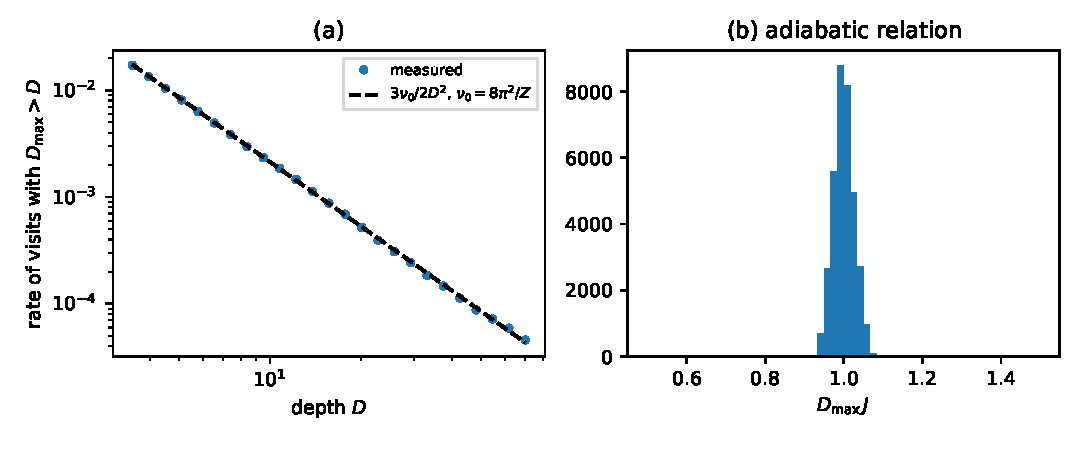
\includegraphics[width=.85\textwidth]{fig_nu0.pdf}
\caption{Channel statistics of pure Yang--Mills mechanics at $E=1$ ($512$ trajectories,
$2900$ time units each, $35\,585$ channel visits). (a) Rate of visits to any channel reaching
depth $D_{\max}>D$, against the parameter-free prediction $3\nu_0/2D^2$ with $\nu_0=8\pi^2/Z$.
(b) The adiabatic relation $D_{\max}J=1$ at entry.}
\label{fig:nu0}
\end{figure}

If the flow is ergodic, $\nu_0$ is a microcanonical flux and needs no dynamics. On the surface
$|x|=A$, changing transverse variables to actions and angles (unit Jacobian) and using
$\int dp_x\,p_x\,\delta(E_x-p_x^2/2)=1$ for the along-channel flux, the entry-rate density is
$(2\pi)^2/Z$ per channel end, independent of $A$, with two ends per channel:
\begin{equation}
\nu_0=\frac{8\pi^2}{Z},\qquad Z=\int\delta(1-H)\,d^3q\,d^3p
=4\pi\sqrt2\int\sqrt{1-V(q)}\;\Theta(1-V)\,d^3q .
\end{equation}
$Z$ is the classical density of states of Yang--Mills mechanics at $E=1$, finite despite the open
channels because they narrow as $1/|x|$ (the same integral underlies the discreteness of the
quantum spectrum of the $x^2y^2$ potential \cite{Simon83}). Numerically $Z=557.1$, so
$\nu_0=0.1417$; the measured value from $35\,585$ channel visits is $0.146$ over $D=4$--$16$
(Fig.~\ref{fig:nu0}a), with a slow softening to $\simeq0.12$ at $D=30$--$50$. An independent
re-run with a separately written integrator ($34\,676$ visits) gives $\nu_0=0.140$--$0.146$ over
$D=4$--$16$, $0.134$ at $D=24$--$48$, and $D_{\max}J=0.999$ (median). A larger run
($2048$ trajectories, $T=4000$, $194\,602$ visits) confirms each ingredient of the derivation
separately: $J_{\rm peak}/J_{\rm entry}$ has median $1.000$ (interquartile $0.983$--$1.017$);
$D_{\max}$ against $1/J_{\rm entry}$ has log-log slope $1.00$ and prefactor $1.01$ for visits
deeper than $6$; the cumulative distribution of $J_{\rm entry}$ at small $J$ has slope $2.05$,
i.e.\ a uniform action measure; and the exceedance of $D_{\max}$ has slope $-2.06$. The
deepest recorded visit reached $D=105.6$ over $294.5$ time units with $J_{\rm entry}=0.0095$
and a parabolic profile of the same $J$. The final,
parameter-free result is
\begin{equation}
\boxed{\;\lambda_{\rm diag}(E)=\frac{32\pi^3}{105\sqrt2}\,\frac{E^{9/4}}{Z}\simeq0.0120\,E^{9/4}\;}
\label{eq:final}
\end{equation}
against the measured diagonal-ghost values of Table~\ref{tab:low}: the ratio
measured/predicted is $0.995$, $1.002$, $1.021$, $0.971$ at $E=0.008$, $0.015$, $0.02$, $0.03$
(mean $0.997$, scatter $2\%$), and the free fit (\ref{eq:fit}) gives exponent $2.24\pm0.03$ and,
at fixed $9/4$, prefactor $0.0120\pm0.0003$. Every number on the right-hand side of
(\ref{eq:final}) is either a pure number or the density of states, and the agreement is at the
level of the statistical and extrapolation uncertainties of the measurement. Above the range of
Table~\ref{tab:low} the diagonal rate is $1.10$, $1.10$, $1.09$ times (\ref{eq:final}) at
$E=0.05$, $0.07$, $0.1$, where $u=4.2$--$3.6$ is at the onset of the $u^{-6}$ regime and the
measured spectrum lies slightly above the asymptotic power law, and it falls below
(\ref{eq:final}) from $E\simeq0.15$ on ($0.97$, $0.90$, $0.76$, $0.53$, $0.33$ at $E=0.15$,
$0.2$, $0.3$, $0.5$, $1$), where the resonance has moved into the knee of the spectrum. The
single-mode law therefore holds to $10\%$ over a factor $12$ in energy, $0.008\le E\le0.1$. The resonant depth
at these energies is $D=E^{-1/4}\simeq2.4$--$3.3$, at the lower edge of the range in which the
channel asymptotics were established directly (the $D^{-2}$ plateau of Fig.~\ref{fig:nu0}a
begins at $D\simeq4$); that the law already holds there says the adiabatic description of a visit
is accurate from shallower depths than the plateau test requires. The apparent softening of
$\nu_0$ to $\simeq0.12$--$0.13$ at $D\gtrsim20$ is at the depths where the ensembles run out of
visits (a $D=50$ visit lasts $\sim140$ time units against segments of $410$) and we do not build
on it; if the microcanonical flux is exact, as the derivation assumes, there is nothing to
soften. The remaining factor between the physical vector ghost and the diagonal ghost
($2.2$--$2.3$ at $E=0.015$--$0.03$, $1.75$ at $E=0.008$) is not part of the single-mode argument
and is attributed to interior off-diagonal mixing, where the three modes are degenerate and no
detuning protects them; it falls with energy, and the asymptotic law for the physical ghost is
(\ref{eq:final}) itself.

\section{Nonlinear escape}
\label{sec:nonlinear}

\subsection{Mechanism and time scale}

Full nonlinear evolution on a grid of $(E,\varepsilon)$, with $\varepsilon$ the initial ghost
energy fraction, shows escape to a finite-time singularity in every cell in which escape was
resolved ($E\gtrsim0.06$ at $\varepsilon=10^{-4}$; lower cells were censored by the run length).
Escape times satisfy $t_\esc\lambda_\perp\approx2$--$5\approx\ln(q_{\rm typ}/w_0)$: the linear
instability sets the clock, and the $\varepsilon$-dependence follows
$\tfrac12\ln(1/\varepsilon)$ as expected: the measured shift in $t_\esc\lambda_\perp$ between
$\varepsilon=10^{-4}$ and $10^{-2}$ is $2.3$, against $\tfrac12\ln10^2=2.30$; the re-run at
$E=0.3$ (median $t_\esc=98.5$ and $222.6$ at the two $\varepsilon$, $\lambda_\perp=0.0165$)
gives $2.05$. (The corresponding $E$-dependence, $\tfrac14\ln(1/E)$, has not been checked.)
Adaptive re-integration of escaping trajectories shows that the blow-up is not a clean power law
in the state norm: $|w|,|P|,|W|$ grow monotonically with local per-decade exponents fluctuating
between $\sim1$ and $\sim10$ while $|q|$ is non-monotonic. Sampling the last stretch before
$t_*$ reveals the mechanism: $q$ is thrown along a channel axis with a transverse displacement
$\rho$ for which $1+\lambda_{\min}(\Hess V)=1-3\rho^2\ll0$ (measured $-49.5$ at $\rho=4.11$,
$-160.5$ at $\rho=7.34$); the hugely negative ghost mass matrix drives $w$, and large $w$ drives
$q$ further out. The runaway is a self-accelerating tachyonic loop. The re-run sees the same
sequence in ensemble medians at $E=0.3$: as the largest component passes $10$, $10^2$, $10^3$,
$\rho$ grows $1.0\to1.4\to1.9$, $1+\lambda_{\min}$ falls $-1\to-4\to-9$ (tenth percentile
$-35$) and $|w|$ grows $3\to22\to110$. In pure Yang--Mills the
transverse displacement shrinks with depth adiabatically, which is why the tachyonic fraction
vanishes below $E=\tfrac12$; in the nonlinear runaway the ghost pumps it up. In Smilga's
terminology \cite{Smilga} the ghost is malicious. No polynomial first integral independent of $H$ exists up to degree $4$ in the twelve
phase-space variables (numerical null-space search of $\{H,F\}=0$ over $1820$ monomials, which
recovers exactly the three partial energies for a separable control potential), so none of the
known global-stability mechanisms \cite{DMV22,KLS14} is available at that order.

\subsection{The escape-time landscape}

\begin{figure}
\centering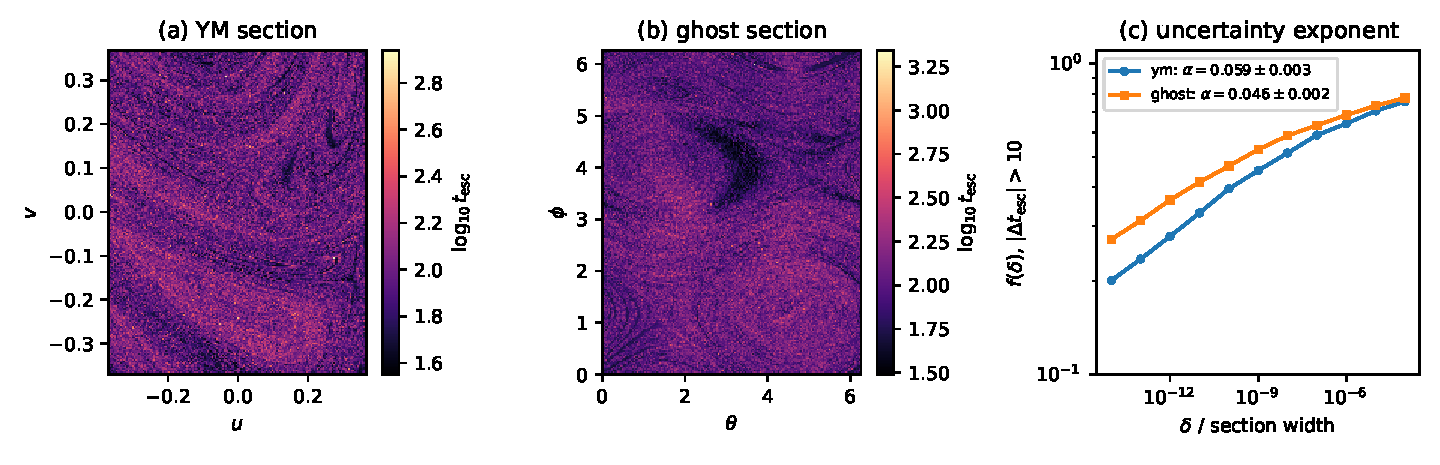
\includegraphics[width=\textwidth]{fig_maps.pdf}
\caption{Escape-time landscape at $E=0.3$, $\varepsilon=0.01$. (a) $256^2$ Yang--Mills section:
the ghost is fixed and the Yang--Mills initial condition is varied over a patch of side $E^{1/4}$
in the $(x,y)$ plane. (b) $256^2$ ghost section: the Yang--Mills point is fixed and the ghost
orientation $(\theta,\phi)$ is varied over the torus. (c) Uncertainty-exponent test: the fraction
$f(\delta)$ of pairs of initial conditions at separation $\delta$ whose escape times differ by
more than $10$ time units, $2\times10^4$ pairs per $\delta$, on both sections.}
\label{fig:maps}
\end{figure}

Since every trajectory escapes, the geometric object is the escape-time function
$t_\esc$(initial condition) and the level sets $\{t_\esc<t\}$. Figure~\ref{fig:maps} shows
$t_\esc$ on two-dimensional sections at $E=0.3$, $\varepsilon=0.01$. Both sections show
stretched and folded bands at large scale, the imprint of the chaotic base flow, on top of a
texture that is rough at the grid scale: neighbouring cells differ in $t_\esc$ by a median of
$30$ time units against a median $t_\esc$ of $95$, and the lag-1 correlation of $\log t_\esc$ is
$0.2$--$0.4$. The ghost section is not smoother in this respect even though the Yang--Mills
initial condition is identical in every cell, because the ghost back-reacts on $q$ at $O(w)$ from
the first step and the base flow amplifies the difference at $\lambda_\YM$; the ghost phase
contributes only a $\pm10\%$ smooth modulation of the median escape time.

The quantitative statement is the uncertainty exponent \cite{GMOY83,BGO90}: for pairs of initial
conditions at separation $\delta$, the fraction $f(\delta)$ whose escape times differ by more
than a threshold scales as $\delta^\alpha$, and the level-set boundaries have dimension
$d=2-\alpha$ on the section. Figure~\ref{fig:maps}c shows $f(\delta)$ over eleven decades, from
$10^{-4}$ to $10^{-14}$ of the section width, with no flattening at the bottom:
\begin{equation}
\alpha_\YM=0.059\pm0.003,\qquad\alpha_{\rm ghost}=0.046\pm0.002\qquad(|\Delta t_\esc|>10),
\end{equation}
and $0.04$--$0.07$ for thresholds between $5$ and $20$ time units. The boundaries of the escape
level sets are fractal with dimension $1.95\pm0.01$ on both sections, essentially area-filling.
The standard chaotic-scattering estimate $\alpha=\kappa/\lambda$ \cite{BGO90}, with
$\kappa=0.027$ the escape rate fitted to the exponential tail of the $t_\esc$ distribution, gives
$\alpha\simeq0.10$ with $\lambda=\lambda_\YM(0.3)=0.28$; the measured value implies an effective
separation rate $\simeq0.5$. A Benettin measurement on the full twelve-dimensional flow at
$\varepsilon=0.01$ ($400$ trajectories, renormalisation every time unit, the last $10$ time
units before escape excluded) gives $\lambda_{\max}=0.33\pm0.01$ as a per-trajectory time
average, against $0.29$ for pure Yang--Mills in the same code: the finite ghost raises the
exponent only modestly, to $\alpha\simeq0.08$. The ensemble-weighted rate
$\sum\ln(\delta/\delta_0)/\sum t=0.42$, which is dominated by the fastest-separating
trajectories, gives $\alpha\simeq0.06$, within the measured range. The small $\alpha$ is thus
mainly a generalised-Lyapunov effect, the escape statistics being controlled by the tail of the
finite-time exponent distribution rather than its mean. Either way, the conclusion is that the set of initial conditions that remain close to
the ghost-free manifold for any prescribed time has no interior: the manifold is a repeller
whose ``basin'' is a fractal of full dimension, at every scale down to the arithmetic.

\section{Invariant sets on which the ghost is bounded}
\label{sec:floquet}

\begin{figure}
\centering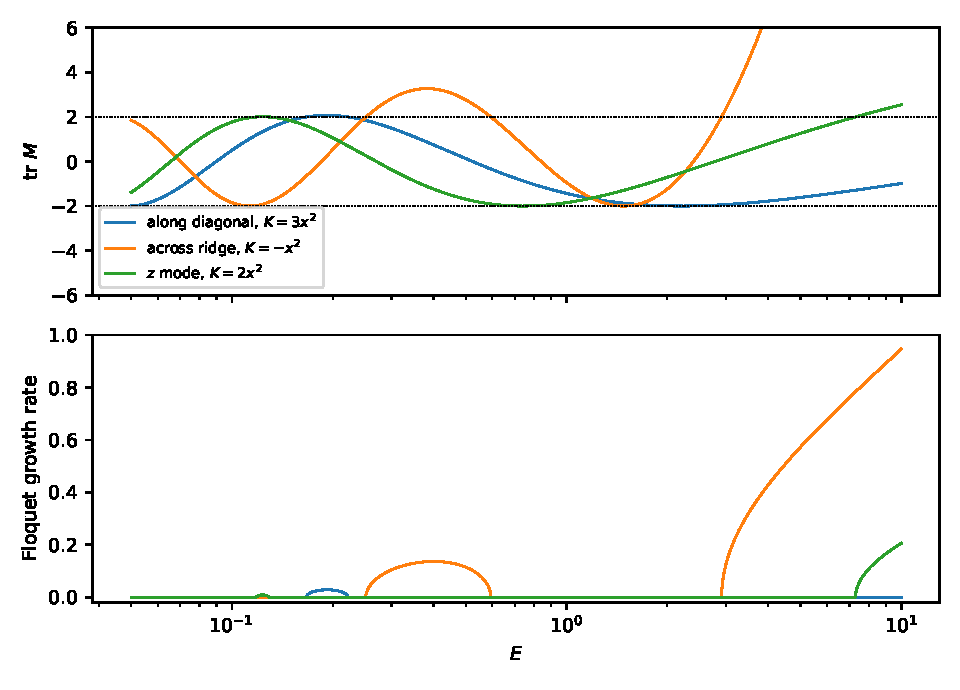
\includegraphics[width=.75\textwidth]{fig_floquet.pdf}
\caption{Floquet stability of the linearised ghost on the diagonal periodic orbit $x=y$, $z=0$
of Yang--Mills mechanics ($\ddot x=-x^3$). The three ghost modes decouple with constant
eigenvectors and $K=3x^2$ (along the diagonal), $-x^2$ (across the ridge, the direction whose
eigenvalue reaches the bound $-\sqrt{2V}$), $2x^2$ ($z$). Top: trace of the monodromy matrix;
bottom: Floquet growth rate.}
\label{fig:floquet}
\end{figure}

In a Hamiltonian system nothing attracts, so the question ``where can a ghost sit'' is a question
about invariant sets on which the linearised ghost is bounded. On a periodic orbit of the base
flow Eq.~(\ref{eq:hill}) is a genuine Hill equation. Figure~\ref{fig:floquet} shows the result on
the diagonal orbit: the ghost is Floquet-stable over most of the energy range, with narrow
instability tongues at $E\in(0.165,0.222)$ (along-diagonal mode), $(0.25,0.585)$ and $E>2.9$
(ridge mode), and $(0.117,0.127)$, $E>7.2$ ($z$ mode). Two points deserve emphasis. First, for
$E\in(0.585,2.9)$ the ghost mass matrix is negative on part of every period yet the ghost is
Floquet-stable: a transiently tachyonic mass is not an instability on a periodic orbit. Second,
at $E=0.3$ the ridge mode on this orbit grows at rate $0.11$--$0.13$, six to ten times the
chaotic-average $\lambda_\perp$; this orbit is the ridge on which the tachyonic configurations of
Sec.~\ref{sec:model} live, and the lower edge of its tongue, $E=0.25$, coincides with the end of
the steepening of $\lambda_\perp(E)$. Whether this is more than a coincidence requires the same
analysis on the other short periodic orbits (the channel and ``circular'' orbits), which we have
not carried out. All such
orbits are hyperbolic within the base flow, so these are landing points for the ghost but not
for the trajectory: saddles within a saddle, of measure zero twice over. The only candidate for a
positive-measure set on which the ghost stays bounded is the regular islands of Yang--Mills
mechanics \cite{DahlqvistRussberg}, on which the driving is quasi-periodic; whether any survive in
the three-component system with a ghost attached is open.

\section{Discussion}
\label{sec:discussion}

\paragraph{Scope.} Instability of an exact sector implies instability of the full classical
Lee--Wick Yang--Mills theory on $T^3$, as an existence statement. The torus is also what makes
the homogeneous sector physically meaningful rather than a formal truncation: the inhomogeneous
modes carry momenta $\ge2\pi/L$, and on a small torus ($L$ below the inverse field strength)
they are gapped and the zero-momentum sector dominates the low-energy dynamics
\cite{Luscher83}. On a large torus the homogeneous Yang--Mills condensate is itself unstable to
inhomogeneous modes at rates of order $\lambda_\YM$, which at low energy vastly exceeds
$\lambda_\perp$; a real homogeneous configuration then fragments and thermalises long before its
ghost grows, and the relevant follow-up is ghost growth in a thermal-like
Yang--Mills state, for which the lattice machinery of glasma-instability studies exists
\cite{MullerTrayanov,Kunihiro}. Nothing here addresses the quantum theory directly.

\paragraph{The fakeon classical limit.} In the fakeon prescription the classical limit is
defined by solving the ghost equation with the half-retarded, half-advanced Green function and
substituting back, which discards precisely the homogeneous solutions of (\ref{eq:hill})
\cite{Anselmi18}. The ghost-free manifold $w=W=0$ is that projection at leading order. Our
results say that this manifold is a repeller at every energy, with polynomially short growth
times, and that its ``basin'' has no interior. The projection is therefore a definition rather
than a dynamical statement: the classical projected theory is not the limit of nearby classical
solutions, and any perturbation at the level of $10^{-12}$ of the initial data lands in the
fractal. This does not refute the prescription, which is a statement about the quantum theory and
need not have a classical limit in this sense, but it identifies the question a consistent
classical limit must answer: what principle keeps the system on a measure-zero repelling manifold.

\paragraph{Contrast with benign ghosts.} The globally stable and benign ghost systems in the
literature \cite{DMV22,DamourSmilga,Smilga} have interactions chosen for stability, and several
are integrable or nearly so. Here the interactions are fixed by gauge symmetry and the normal
sector is chaotic, and the ghost is malicious. We conjecture that a ghost coupled to a chaotic
normal sector is never benign: the argument of Sec.~\ref{sec:derivation} needs only a chaotic base
flow whose phase-space measure near the resonant configurations is a power law, which is generic.
This is testable in the existing toy models by adding a chaotic term. Salvio's metastability
thresholds \cite{Salvio19} in interacting Pais--Uhlenbeck-type systems are the natural contrast to
the absence of any threshold here.

\paragraph{Cosmological scaling.} The natural energy unit $M^4/g^2$ translates, for the
gravitational case, to $E\sim\rho/(m_\chi^2M_P^2)\sim H^2/m_\chi^2$ with $m_\chi$ the ghost mass:
the Einstein--Hilbert normalisation $M_P^2$ plays the role of $1/g^2$ and the ghost mass that of
$M$, so this is dimensional matching, not a derived correspondence. Today, for a ghost mass
within a few orders of the Planck mass,
$E\sim10^{-120}$ and (\ref{eq:final}) gives a growth rate of order $10^{-270}m_\chi$: the absence
of exponential suppression is irrelevant in practice, and the classical ghost is harmless at all
post-inflationary energies. The crossover $E\sim\tfrac12$ corresponds to $H\sim m_\chi$, i.e.\ to
inflation if the ghost mass is comparable to the Hubble rate then, which is the regime in which
the fakeon consistency bound $m_\chi\gtrsim m_\phi/4$ of \cite{ABP20} must hold. The classical
tachyonic threshold and the quantum consistency bound are the same line seen from two sides; the
passage through it at the end of inflation is the one epoch at which the nonlinear dynamics
studied here could have mattered.

\paragraph{Open items.} (i) The vector/diagonal factor ($\simeq2.2$ at $E=0.015$--$0.03$,
$1.75$ at $E=0.008$): a derivation of the mode-mixing contribution and of the rate at which it
dies off, which would turn the asymptotic statement into a prediction for the physical ghost at
all $E\lesssim0.03$. (ii) The two-field $x^2y^2$ model, for which the same argument predicts
$\lambda\propto E^{2}$ (one transverse action instead of two): a cheap and pointed test of the
decomposition of the exponent. (iii) The finite-time Lyapunov distribution of the full flow,
whose tail sets $\alpha$ (Sec.~\ref{sec:nonlinear}). (iv) The regular islands as a possible
positive-measure refuge. (v) Bianchi IX minisuperspace of quadratic gravity, in which the same
calculation can be done for the theory of actual interest.

\section*{Acknowledgements}
The numerical code, the derivations of Sec.~\ref{sec:derivation}, and much of the analysis in
this paper were developed in interactive sessions with Claude (Anthropic). The choice of problem,
the numerical experiments, and the judgement calls throughout are the author's, as is
responsibility for any errors.

\begin{thebibliography}{99}
\small
\bibitem{Stelle77} K.~S.~Stelle, Phys.\ Rev.\ D {\bf 16}, 953 (1977).
\bibitem{Anselmi17} D.~Anselmi, JHEP {\bf 06}, 086 (2017), arXiv:1704.07728.
\bibitem{Anselmi18} D.~Anselmi, JHEP {\bf 02}, 141 (2018), arXiv:1801.00915; Class.\ Quantum Grav.\ {\bf 36}, 065010 (2019), arXiv:1809.05037.
\bibitem{ABP20} D.~Anselmi, E.~Bianchi and M.~Piva, JHEP {\bf 07}, 211 (2020), arXiv:2005.10293.
\bibitem{LeeWick} T.~D.~Lee and G.~C.~Wick, Nucl.\ Phys.\ B {\bf 9}, 209 (1969); Phys.\ Rev.\ D {\bf 2}, 1033 (1970).
\bibitem{GOW08} B.~Grinstein, D.~O'Connell and M.~B.~Wise, Phys.\ Rev.\ D {\bf 77}, 025012 (2008).
\bibitem{DonoghueMenezes} J.~F.~Donoghue and G.~Menezes, Phys.\ Rev.\ D {\bf 100}, 105006 (2019), arXiv:1908.02416; Phys.\ Rev.\ Lett.\ {\bf 123}, 171601 (2019), arXiv:1908.04170.
\bibitem{SalvioStrumia} A.~Salvio and A.~Strumia, JHEP {\bf 06}, 080 (2014); A.~Salvio, Front.\ Phys.\ {\bf 6}, 77 (2018).
\bibitem{Salvio19} A.~Salvio, Phys.\ Rev.\ D {\bf 99}, 103507 (2019), arXiv:1902.09557.
\bibitem{DMV22} C.~Deffayet, S.~Mukohyama and A.~Vikman, Phys.\ Rev.\ Lett.\ {\bf 128}, 041301 (2022), arXiv:2108.06294; C.~Deffayet, A.~Held, S.~Mukohyama and A.~Vikman, JCAP {\bf 11}, 031 (2023), arXiv:2305.09631; Phys.\ Rev.\ D {\bf 112}, 065011 (2025), arXiv:2504.11437.
\bibitem{DamourSmilga} T.~Damour and A.~Smilga, Phys.\ Rev.\ D {\bf 105}, 045018 (2022), arXiv:2110.11175.
\bibitem{Smilga} A.~V.~Smilga, Int.\ J.\ Mod.\ Phys.\ A {\bf 32}, 1730025 (2017), and references therein.
\bibitem{KLS14} D.~S.~Kaparulin, S.~L.~Lyakhovich and A.~A.~Sharapov, Eur.\ Phys.\ J.\ C {\bf 74}, 3072 (2014).
\bibitem{note:derive} The reduction, its consistency (Gauss law and off-diagonal equations vanish on the ansatz), symmetric criticality, and the auxiliary-field form were verified symbolically with \texttt{hdym\_derive.py} in the repository of Sec.~\ref{sec:methods}, \url{https://github.com/foejoseph-lab/hdym}.
\bibitem{MatinyanSavvidy} S.~G.~Matinyan, G.~K.~Savvidy and N.~G.~Ter-Arutyunyan-Savvidy, Sov.\ Phys.\ JETP {\bf 53}, 421 (1981).
\bibitem{Savvidy} G.~K.~Savvidy, Nucl.\ Phys.\ B {\bf 246}, 302 (1984).
\bibitem{Luscher83} M.~L\"uscher, Nucl.\ Phys.\ B {\bf 219}, 233 (1983).
\bibitem{DahlqvistRussberg} P.~Dahlqvist and G.~Russberg, Phys.\ Rev.\ Lett.\ {\bf 65}, 2837 (1990).
\bibitem{Simon83} B.~Simon, Ann.\ Phys.\ {\bf 146}, 209 (1983).
\bibitem{Yoshida} H.~Yoshida, Phys.\ Lett.\ A {\bf 150}, 262 (1990).
\bibitem{OttSommerer} E.~Ott and J.~C.~Sommerer, Phys.\ Lett.\ A {\bf 188}, 39 (1994).
\bibitem{ABS96} P.~Ashwin, J.~Buescu and I.~Stewart, Nonlinearity {\bf 9}, 703 (1996).
\bibitem{APW86} L.~Arnold, G.~Papanicolaou and V.~Wihstutz, SIAM J.\ Appl.\ Math.\ {\bf 46}, 427 (1986).
\bibitem{Jarzynski93} C.~Jarzynski, Phys.\ Rev.\ E {\bf 48}, 4340 (1993).
\bibitem{Ott79} E.~Ott, Phys.\ Rev.\ Lett.\ {\bf 42}, 1628 (1979).
\bibitem{Neishtadt} A.~I.~Neishtadt, J.\ Appl.\ Math.\ Mech.\ {\bf 48}, 133 (1984).
\bibitem{GMOY83} C.~Grebogi, S.~W.~McDonald, E.~Ott and J.~A.~Yorke, Phys.\ Lett.\ A {\bf 99}, 415 (1983).
\bibitem{BGO90} S.~Bleher, C.~Grebogi and E.~Ott, Physica D {\bf 46}, 87 (1990).
\bibitem{MullerTrayanov} B.~M\"uller and A.~Trayanov, Phys.\ Rev.\ Lett.\ {\bf 68}, 3387 (1992).
\bibitem{Kunihiro} T.~Kunihiro, B.~M\"uller, A.~Ohnishi, A.~Sch\"afer, T.~T.~Takahashi and A.~Yamamoto, Phys.\ Rev.\ D {\bf 82}, 114015 (2010).
\end{thebibliography}

\end{document}
